\subsection{I/O FROM LOCAL DISK}
The first set of experiments are a set of simple, single-machine experiments. The goal is to examine how the various complex object implementations compare for a simple from-disk retrieval task. In this set of experiments, the part, tweet data set is first loaded onto the HDD drive of a single machine—one version for each of the ten complex object implementations tested–where they are organized into $256KB$ pages. The objects are then indexed, using a dense index.

Two experiments are run. In the first, a particular object is looked up in the index, and then enough pages are read from disk to access that object, as well as the following $n − 1$ objects. As the pages are loaded into RAM, all n objects are deserialized and made ready for processing. This tests the ability of the object implementation to support fast processing of objects in sequence. We test $n$ in \{  $1\times 10^6$ , $2\times10^6$, $3\times10^6$, $4\times10^6$, $5\times10^6$ \}.

In the second experiment, a list of n, randomly-selected objects are accessed, in order. For each object, the location of the object in the database is looked up in the index, and then the corresponding page is loaded into RAM. The desired object is then deserialized from the page. This simulates a scenario where objects are retrieved from secondary storage using a secondary index.

Before the experiment, the operating system buffer cache is emptied. We do not utilize a dedicated buffer cache, but we do allow the operating system to cache disk pages.

One concern is that since there was only one thread active at a given time during each experiment, this might give an unfair advantage to those solutions running in the JVM. One of the classical performance problems observed during garbage collection is long pauses during which worker threads are largely locked out of allocations. When only a single thread is available, serial execution is already forced, and hence the cost
of such a pause is minimized. A single-threaded environment might also give an unfair advantage to the non-in-place C++ solutions, as $malloc()$ and $free()$ may be less of a bottleneck when only a single thread is running. Hence, we also ran a set of sequential read experiments where four threads
we allowed to concurrently read and then process different ranges of the required data. This may give a better idea of the performance in a realistic, multi-threaded environment.

\subsubsection{Results}
\begin{figure}
	\centering
	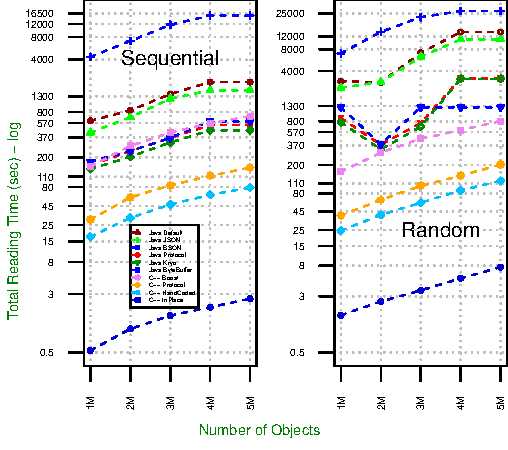
\includegraphics[width=\columnwidth,height=4.5cm,keepaspectratio]{img/Experiment_ReadObjects_CPU.pdf}
	\caption{sequential and random read}
	\label{fig:sequental_random_read}
\end{figure}

\subsubsection{Discussion}
